\documentclass{report}
\usepackage[T1]{fontenc} % Fontes T1
\usepackage[utf8]{inputenc} % Input UTF8
\usepackage[backend=biber, style=ieee]{biblatex} % para usar bibliografia
\usepackage{csquotes}
\usepackage[portuguese]{babel} %Usar língua portuguesa
\usepackage{blindtext} % Gerar texto automaticamente
\usepackage[printonlyused]{acronym}
\usepackage{hyperref} % para autoref
\usepackage{graphicx}
\usepackage{indentfirst}
\usepackage{multicol}
\usepackage{ragged2e}
\usepackage{textcomp}

\bibliography{bibliografia}


\begin{document}
%%
% Definições
%
\def\titulo{PROJETO FINAL}
\def\data{DATA}
\def\autores{Bruno Pereira, Tiago Ferreira, Tiago Garcia, Rúben Gomes}
\def\autorescontactos{(112726) \href{mailto:brunoborlido@ua.pt}{brunoborlido@ua.pt}, (112787) \href{mailto:taof@ua.pt}{taof@ua.pt}\\(114184) \href{mailto:tiago.rgarcia@ua.pt}{tiago.rgarcia@ua.pt}, (113435) \href{mailto:rlcg@ua.pt}{rlcg@ua.pt}}
\def\versao{VERSAO 1}
\def\departamento{Dept. de Eletrónica, Telecomunicações e Informática}
\def\empresa{Universidade de Aveiro}
\def\logotipo{../images/ua.pdf}
%
%%%%%% CAPA %%%%%%
%
\begin{titlepage}

\begin{center}
%
\vspace*{50mm}
%
{\Huge \titulo}\\ 
%
\vspace{10mm}
%
{\Large \empresa}\\
%
\vspace{10mm}
%
{\LARGE \autores}\\ 
%
\vspace{30mm}
%
\begin{figure}[h]
\center
\includegraphics{\logotipo}
\end{figure}
%
\vspace{30mm}
\end{center}
%
\begin{flushright}
\versao
\end{flushright}
\end{titlepage}

%%  Página de Título %%
\title{%
{\Huge\textbf{\titulo}}\\
{\Large \departamento\\ \empresa}
}
%
\author{%
    \autores \\
    \autorescontactos
}
%
\date{\today}
%
\maketitle

\pagenumbering{roman}

%%%%%% RESUMO %%%%%%
\begin{abstract}
    O segunte relatório tem como objetivo apresentar o desenvolvimento de um website interativo, com várias funcionalidades.\ Este projeto foi realizado no âmbito da unidade curricular de \ac{labi} do curso de \ac{leci} da \ac{ua}.\\
    Neste relatório, são apresentadas as linguagens utilizadas, as funcionalidades implementadas, as dificuldades encontradas e os resultados obtidos.\\
    Os autores deste projeto são Bruno Pereira, Tiago Ferreira, Tiago Garcia e Rúben Gomes, sendo todos alunos do curso de \ac{leci} da \ac{ua}.\ As contribuições de cada membro do grupo estão descritas no \autoref{chap.analise}.
    Com o seguinte projeto, os autores pretendem demonstrar os conhecimentos adquiridos ao longo do semestre, e também, a capacidade de trabalhar em grupo.

\end{abstract}


%%%%%% Agradecimentos %%%%%%
% Segundo glisc deveria aparecer após conclusão...
%\renewcommand{\abstractname}{Agradecimentos}
%\begin{abstract}
%Eventuais agradecimentos.
%Comentar bloco caso não existam agradecimentos a fazer.
%\end{abstract}


\tableofcontents
% \listoftables     % descomentar se necessário
\listoffigures    % descomentar se necessário


%%%%%%%%%%%%%%%%%%%%%%%%%%%%%%%
\clearpage
\pagenumbering{arabic}

%%%%%%%%%%%%%%%%%%%%%%%%%%%%%%%%
\chapter{Introdução}
\label{chap.introducao}

Este projeto visa implementar um website interativo com várias funcionalidades, sendo estas, por exemplo, a criação de um utilizador, upload de imagens, sistema de comentário e likes/dislikes, entre outros. \\

O site tem como base o \textit{cherrypy}, cujo é responsável pela lógica/ligação entre as páginas em si.\ Também tem outro papel bastante importante, que é realizar a ligação de métodos \textit{post/get} do servidor, e o \ac{js} da página, para ser apresentado dados em tempo real na página.\\

Também é usado uma base de dados em \ac{sql}, com múltiplas tabelas.\ Cada uma tem a sua finalidade, como, por exemplo, guardar as credenciais de um utilizador, comentários de uma imagem, etc.

O site está repartido em várias páginas, sendo estas:
\begin{itemize}
    \item \textbf{index.html} - Página inicial do site, onde é possível fazer login e criar conta
    \item \textbf{upload.html} - Página onde é possível fazer upload de imagens.
    \item \textbf{image.html} - Página onde se pode ver uma imagem em específico, com os seus comentários e likes/dislikes.
    \item \textbf{profile.html} - Página onde é possível ver o perfil de um utilizador.
    \item \textbf{main.html} - Página onde é possível ver os destaques das imagens na base de dados.
    \item \textbf{gallery.html} - Página onde é possível ver as imagens que o utilizador deu like.
    \item \textbf{about.html} - Página onde é possível ver informações sobre os respetivos autores.
\end{itemize}

Cada página será explicada em detalhe mais adiante.\\

Este documento está dividido em quatro capítulos.\\

Depois desta introdução,
no \autoref{chap.metodologia} é apresentada a metodologia seguida,
no \autoref{chap.resultados} são apresentados os resultados obtidos,
sendo estes discutidos no \autoref{chap.analise}.
Finalmente, no \autoref{chap.conclusao} são apresentadas
as conclusões do trabalho.

\chapter{Metodologia}
\label{chap.metodologia}
    Foi utilizada uma metodologia de desenvolvimento incremental, onde cada membro do grupo ficou responsável por uma parte do site.\ Deste modo, foi possível desenvolver o site de forma mais rápida e eficiente.\\

\section{Linguagens usadas}\label{sec:linguagens-usadas}
    As linguagens usadas para o desenvolvimento do site foram \ac{html}, \ac{css}, \ac{js}, \ac{sql} e \textit{python}.\ O \ac{html} foi usado para a estrutura das páginas do site, o \ac{css} para a sua aparência, o \ac{js} para a interação do utilizador com o site, o \ac{sql} para a base de dados, e o \textit{python} para a coligação lógica entre todos os componentes.\\

\subsection{JS}\label{subsec:js}
    A linguagem \ac{js} foi usada para a interação do utilizador com o site, sendo esta responsável por fazer pedidos ao servidor, e receber informação do mesmo.\ Também é responsável por fazer a validação de dados, como, por exemplo, se o utilizador introduziu um email válido.\ A informação é enviada para o servidor através de pedidos \textit{post}, e é recebida através de pedidos \textit{get}, em formato \ac{json}.\ O \ac{js} também é responsável por fazer a ligação entre o \textit{python} e o \ac{html}, sendo este responsável por atualizar a página em tempo real, sem ser necessário fazer \textit{refresh} à página.\\

\subsection{Python}\label{subsec:python}
    A linguagem de programação \textit{python} foi usada especialmente para a ligação entre o \ac{js} e o \ac{sql}, sendo feito o processamento de informação vinda do website para poder realizar pedidos à base de dados, e vice-versa.\ O \textit{python} foi usado com o \textit{cherrypy}, uma framework para a criação de aplicações web, para ser possível processar pedidos \textit{post/get} do servidor.

\section{Base de dados}\label{sec:base-de-dados}
    A base de dados foi feita em \ac{sql}, e tem várias tabelas, sendo estas:
    \begin{itemize}
        \item \textbf{users} - Tabela responsável por guardar as credenciais de um utilizador.
        \item \textbf{images} - Tabela responsável por guardar as imagens.
        \item \textbf{comments} - Tabela responsável por guardar os comentários de uma imagem.
        \item \textbf{votes} - Tabela responsável por guardar os likes/dislikes de uma imagem.
    \end{itemize}
    No~\ref{chap.analise}, é apresentado o esquema da base de dados, com as respetivas tabelas e colunas.

\newpage

%\subsection{Utilização de acrónimos}
%Esta é a primeira invocação do acrónimo \ac{ua}.
%E esta é a segunda \ac{ua}.
%
%Outra referência à \ac{leci}.

\section{Referências bibliográficas}\label{sec:referencias-bibliograficas}
Informação relativa à estrutura formal de um relatório pode ser obtida
na página do \ac{glisc}\cite{glisc}.

\chapter{Resultados}
\label{chap.resultados}

\section {Estrutura do Projeto}\label{sec:estrutura-do-projeto}

O projeto é constituido por :

\begin{itemize}
    \item Pasta "HTML" com os ficheiros HTML do projeto.
    \item Pasta "CSS" com os ficheiros CSS do projeto.
    \item Pasta "JS" com os ficheiros JavaScript do projeto.
    \item Pasta "Images" com as imagens utilizadas na elaboração do site.
    \item Pasta "tmp" com os ficheiros temporários do projeto.
    \item Pasta "uploads" com as imagens enviadas pelos utilizadores.
    \item Ficheiro Python "app.py" define a estrutura de uma aplicação web.
    \item Ficheiro MySQLite "database.sql" que define a estrutura de uma base de dados.
    \item Base de Dados "database.db" que armazena todas as informaçoẽs obtidas através do site.
\end{itemize}

\section {Estrutura do Site}\label{sec:estrutura-do-site}

\indent O site é constituido por 7 páginas iteráveis, sendo elas:

\subsubsection{index.html - Login/Register}

\indent Esta página é a primeira página do site, onde o utilizador pode fazer login ou registar-se no caso de não ter conta.Aqui o utilizador através do nome de utilizador ou pelo email, também pode recuperar a sua password no caso de não se recordar dela.\\


\subsubsection{main.html - Main Page}

\indent Esta página é a página principal do site, onde o utilizador vai ver as com mais gostos comentarios que foram publicadas por ele e outros utilizadores.\\


\subsubsection{galery.html - Gallery}

\indent Esta página é a galeria de imagens do site, onde o utilizador tem acesso a todas as imagens publicadas por ele ou outros utilizadores.\\

\subsubsection{uploads.html - Uploads}

\indent Esta página é a página de uploads do site, onde o utilizador fornece um nome para a imagem bem como o seu autor e então opode publica-la no site.\\

\subsubsection{profile.html - Profile}

\indent Esta página é o perfil do utilizador, onde o utilizador pode ver as imagens que publicou, as imagens que assinalou como favorito e as suas informações.\\
\indent Nesta pagina o utilizador pode alterar as suas informações, como o seu nome, email, password, número de telefone, imagem de perfil, cidade e distrito a que pertence e escrever um pequeno texto que é mostrado no seu perfil.Exite  também uma botão de acesso rapido à página uploads.\\


\subsubsection{image.html - Image}

\indent Esta página é a página de uma imagem, onde o utilizador pode ver a imagem  e as informações da imagem(NomeAutor) para além de poder adicionar à mesma um gosto/desgosto.\\
\indent É aqui que se encontra um botão para adicionar a imagem aos favoritos e uma secção de comentarios disponivel a todos os utilizadores.\\

\subsubsection{about.html - About}

\indent Esta página é a página de informações relacionadas ao site, um link dirigido ao repositório do GitHub, informações sobre os elementos constituintes do grupoe a sua bibliografia e por fim uma imagem do logotipo da Universidade de Aveiro que redireciona o utilizador para a pagina oficial da \acro{UA}.\\

\section {Estrutura da app.py}

\indent O codigo é constituido por 4 partes:

\subsubsection{Configuração de diretórios estáticos:}

\indent As configurações definem os diretórios onde estão localizados os arquivos HTML, JavaScript, CSS, imagens e uploads.Isso permite que o CherryPy sirva esses arquivos estáticos durante a execução do aplicativo.\\

\subsubsection{Classe 'Root'}

\indent É a classe principal que define os manipuladores de URL para diferentes páginas do aplicativo.Cada método decorado com @cherrypy.expose representa uma página acessível pelo URL correspondente.Os métodos retornam o conteúdo dos arquivos HTML correspondentes usando a função open().\\

\subsubsection{Classe 'Actions'}

\indent Essa classe representa ações e manipulações adicionais realizadas no aplicativo.Ela contém métodos decorados com @cherrypy.expose que representam funcionalidades como login, registro, envio de imagens, votação, etc.Os métodos realizam operações no banco de dados SQLite para executar as respectivas ações.\\

\subsubsection{Função 'main'}

\indent É onde a execução do aplicativo é iniciada.O objeto Root é criado e passado como argumento para cherrypy.quickstart(), iniciando o servidor CherryPy e tornando o aplicativo acessível.

\section {Estrutura da database.sql}

\indent A base de dados é constituida por 4 tabelas:

\subsubsection{Users}

\indent Essa tabela provavelmente armazena informações sobre os usuários registrados no aplicativo.
Os campos podem incluir informações como nome, nome de usuário, email e senha.\\

\subsubsection{Images}

\indent Essa tabela provavelmente armazena informações sobre as imagens enviadas pelos usuários.
Os campos podem incluir informações como nome da imagem, autor, caminho do arquivo de imagem, data de criação, etc.\\

\subsubsection{Votes}

\indent Essa tabela provavelmente armazena informações sobre os votos atribuídos às imagens pelos usuários.
Os campos podem incluir informações como ID da imagem relacionada, número de votos positivos (curtidas), número de votos negativos (descurtidas), etc.\\

\subsubsection{Comments}

\indent Essa tabela provavelmente armazena os comentários feitos pelos usuários nas imagens.
Os campos podem incluir informações como ID da imagem relacionada, autor do comentário, texto do comentário, data de criação, etc.\\


\chapter{Análise}
\label{chap.analise}
\section{Site}

\subsubsection{Login/Register}

\begin{figure}[H]
    \centering
    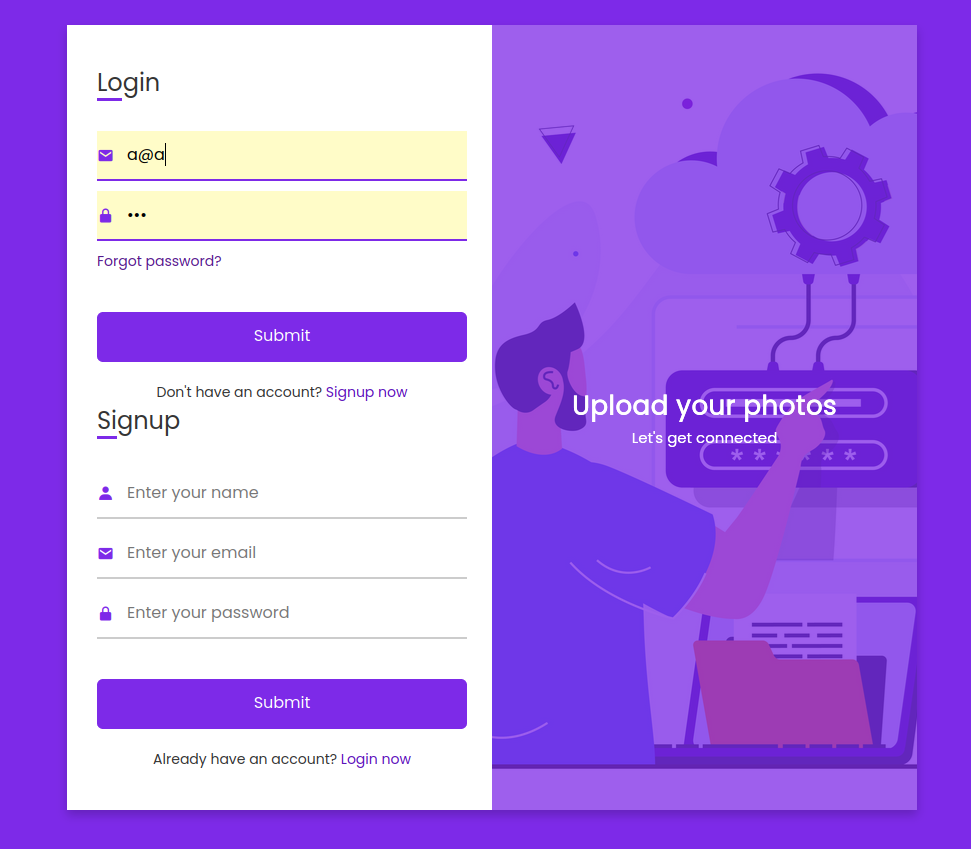
\includegraphics[scale=0.2]{../images/login}
    \caption{Pagina de login}
    \label{fig:login}
\end{figure}

\subsubsection{Main Page}

\begin{figure}[H]
    \centering
    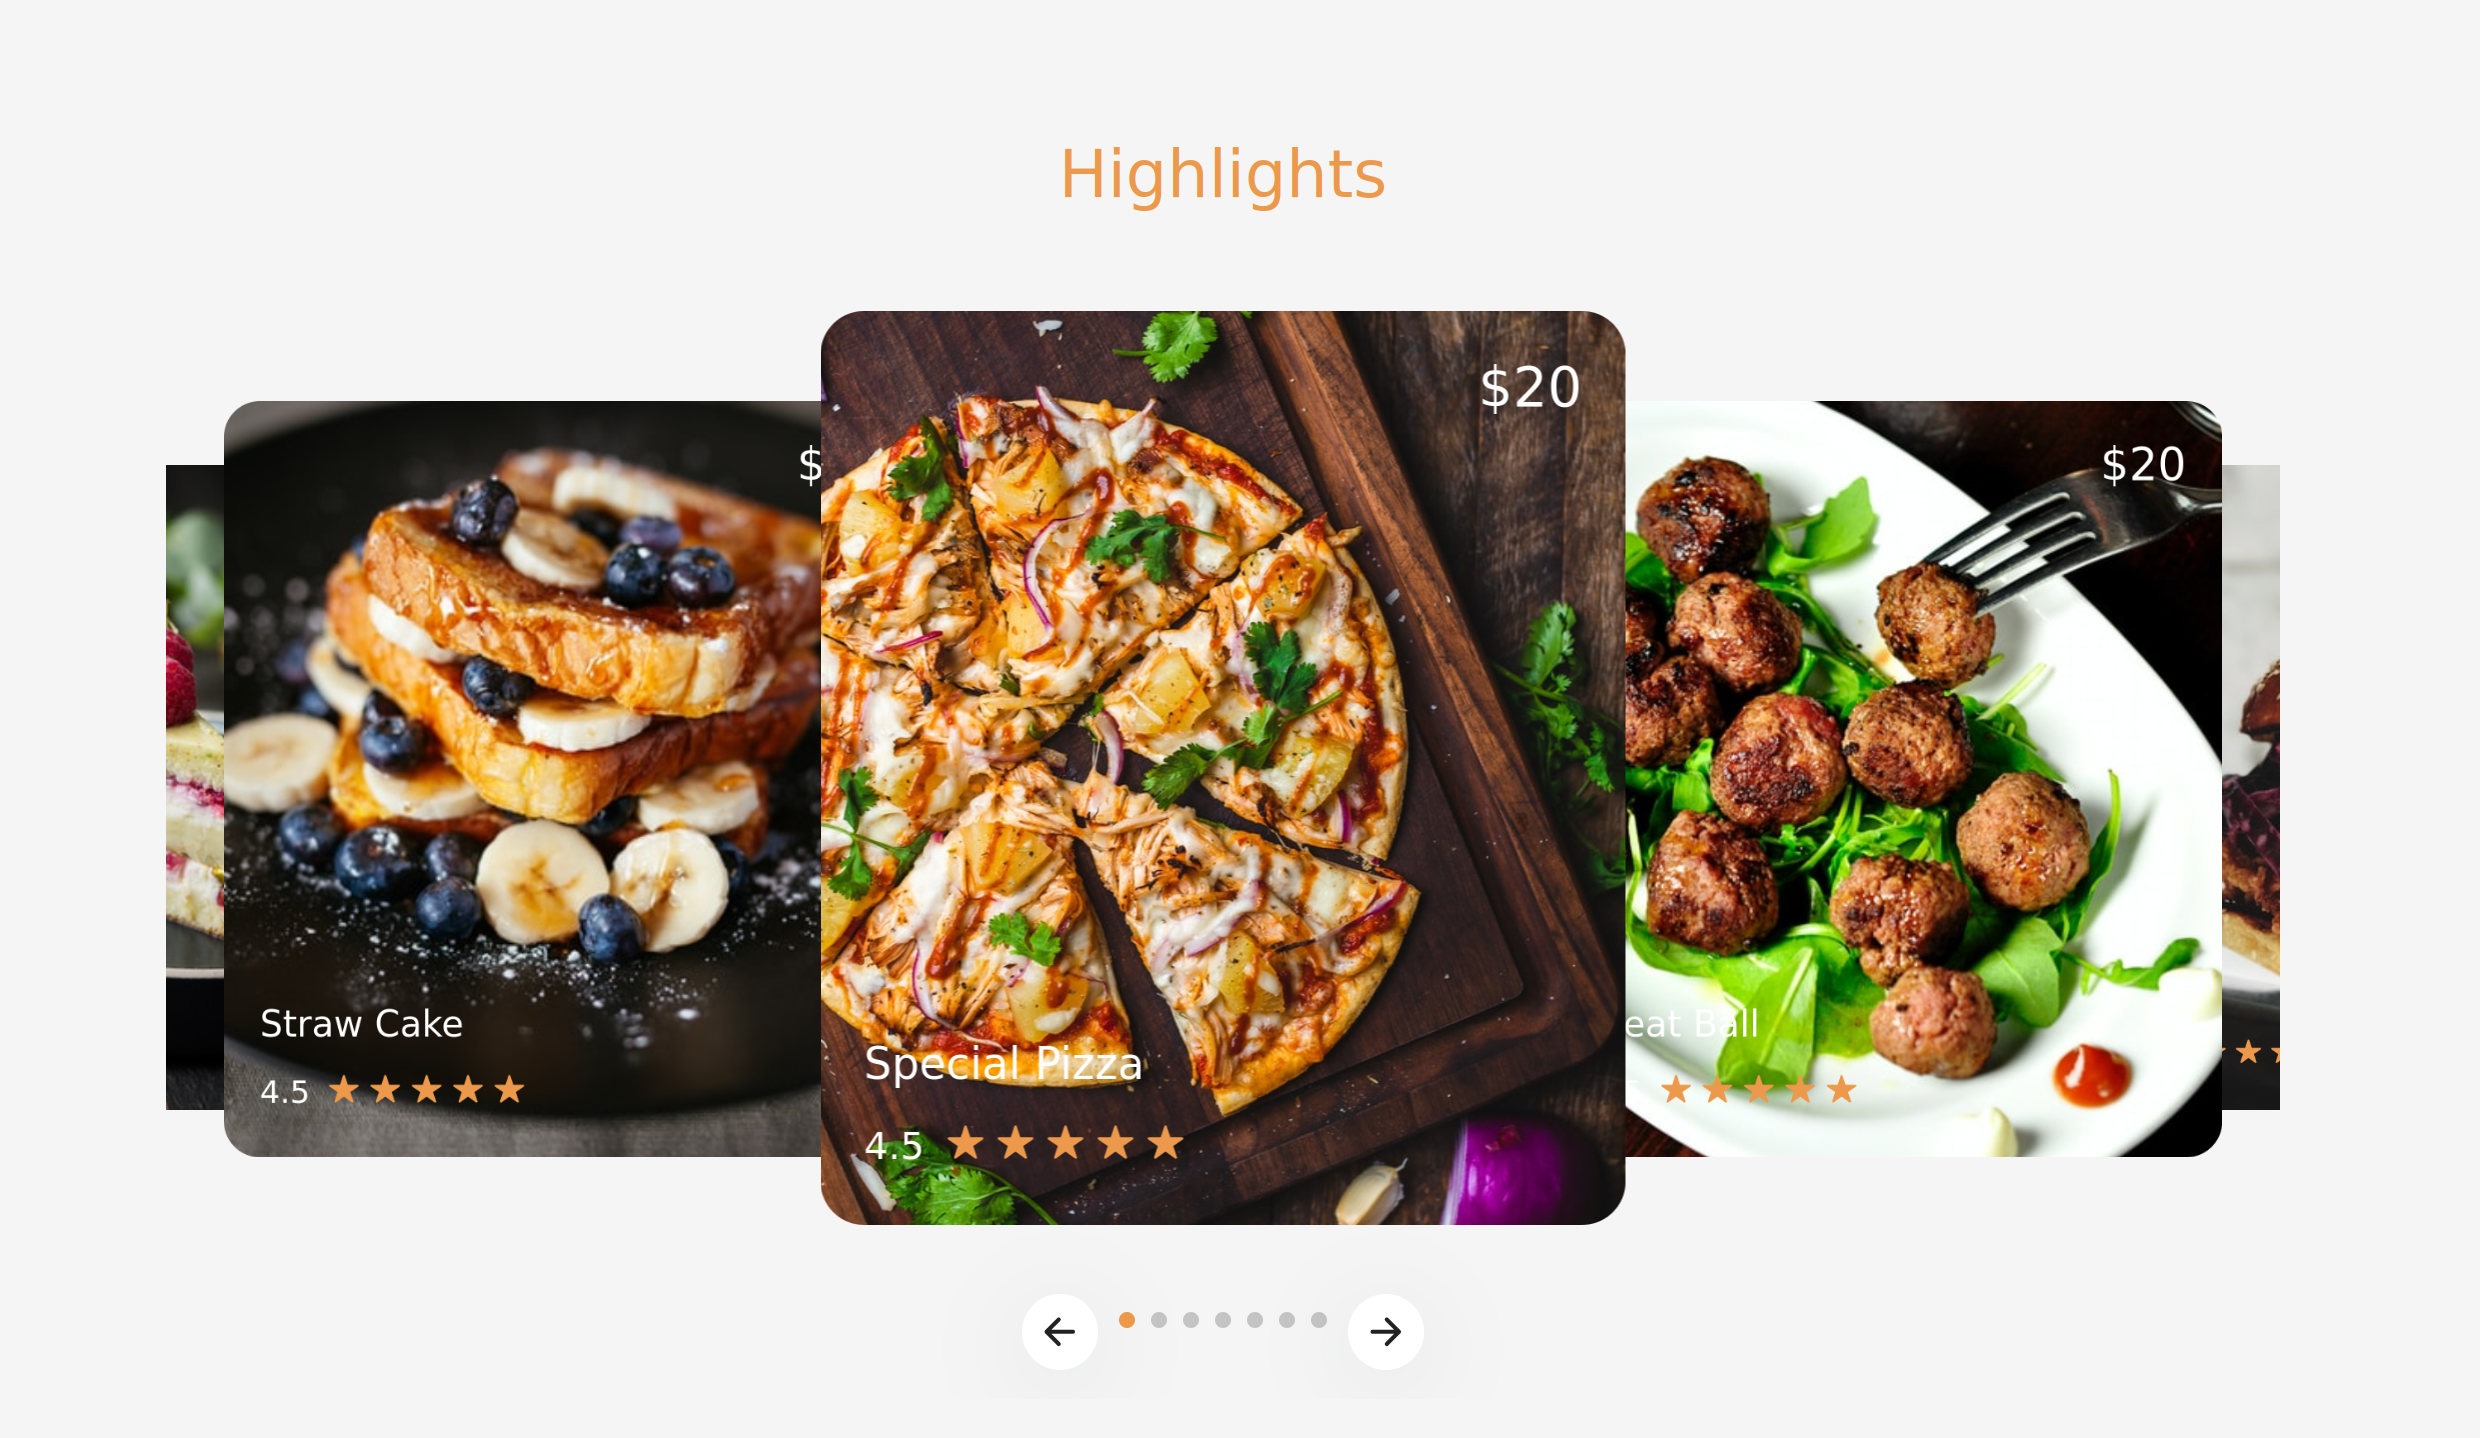
\includegraphics[scale=0.2]{../images/main}
    \caption{Pagina principal}
    \label{fig:Main}
\end{figure}

\subsubsection{Gallery}

\begin{figure}[H]
    \centering
    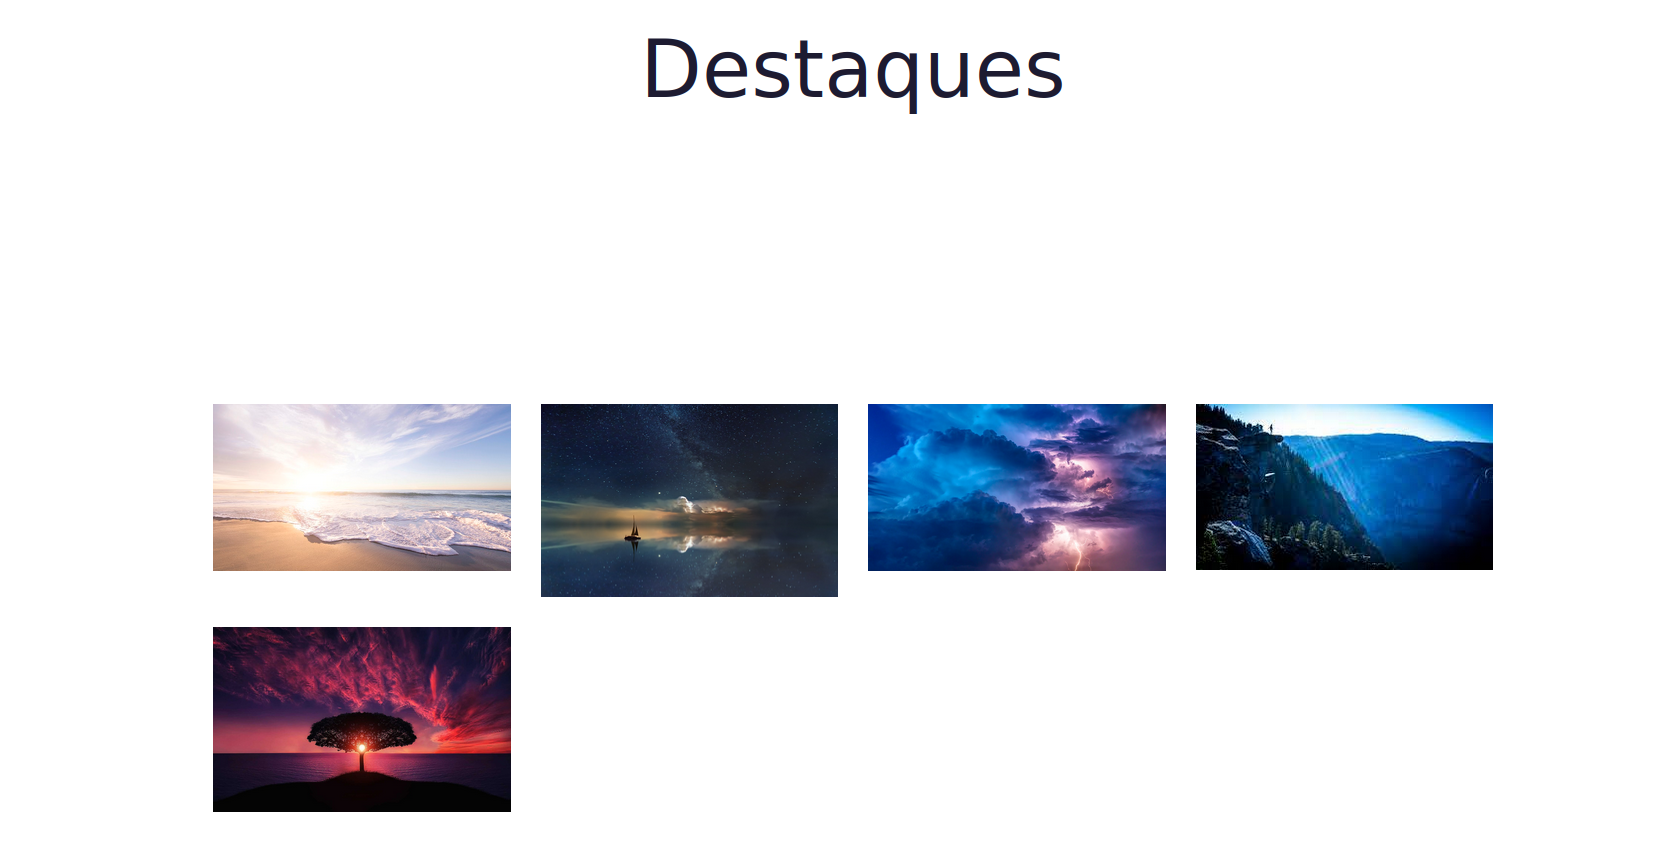
\includegraphics[scale=0.2]{../images/gallery}
    \caption{Pagina de gallery}
    \label{fig:galley }
\end{figure}

\subsubsection{Uploads}

\begin{figure}[H]
    \centering
    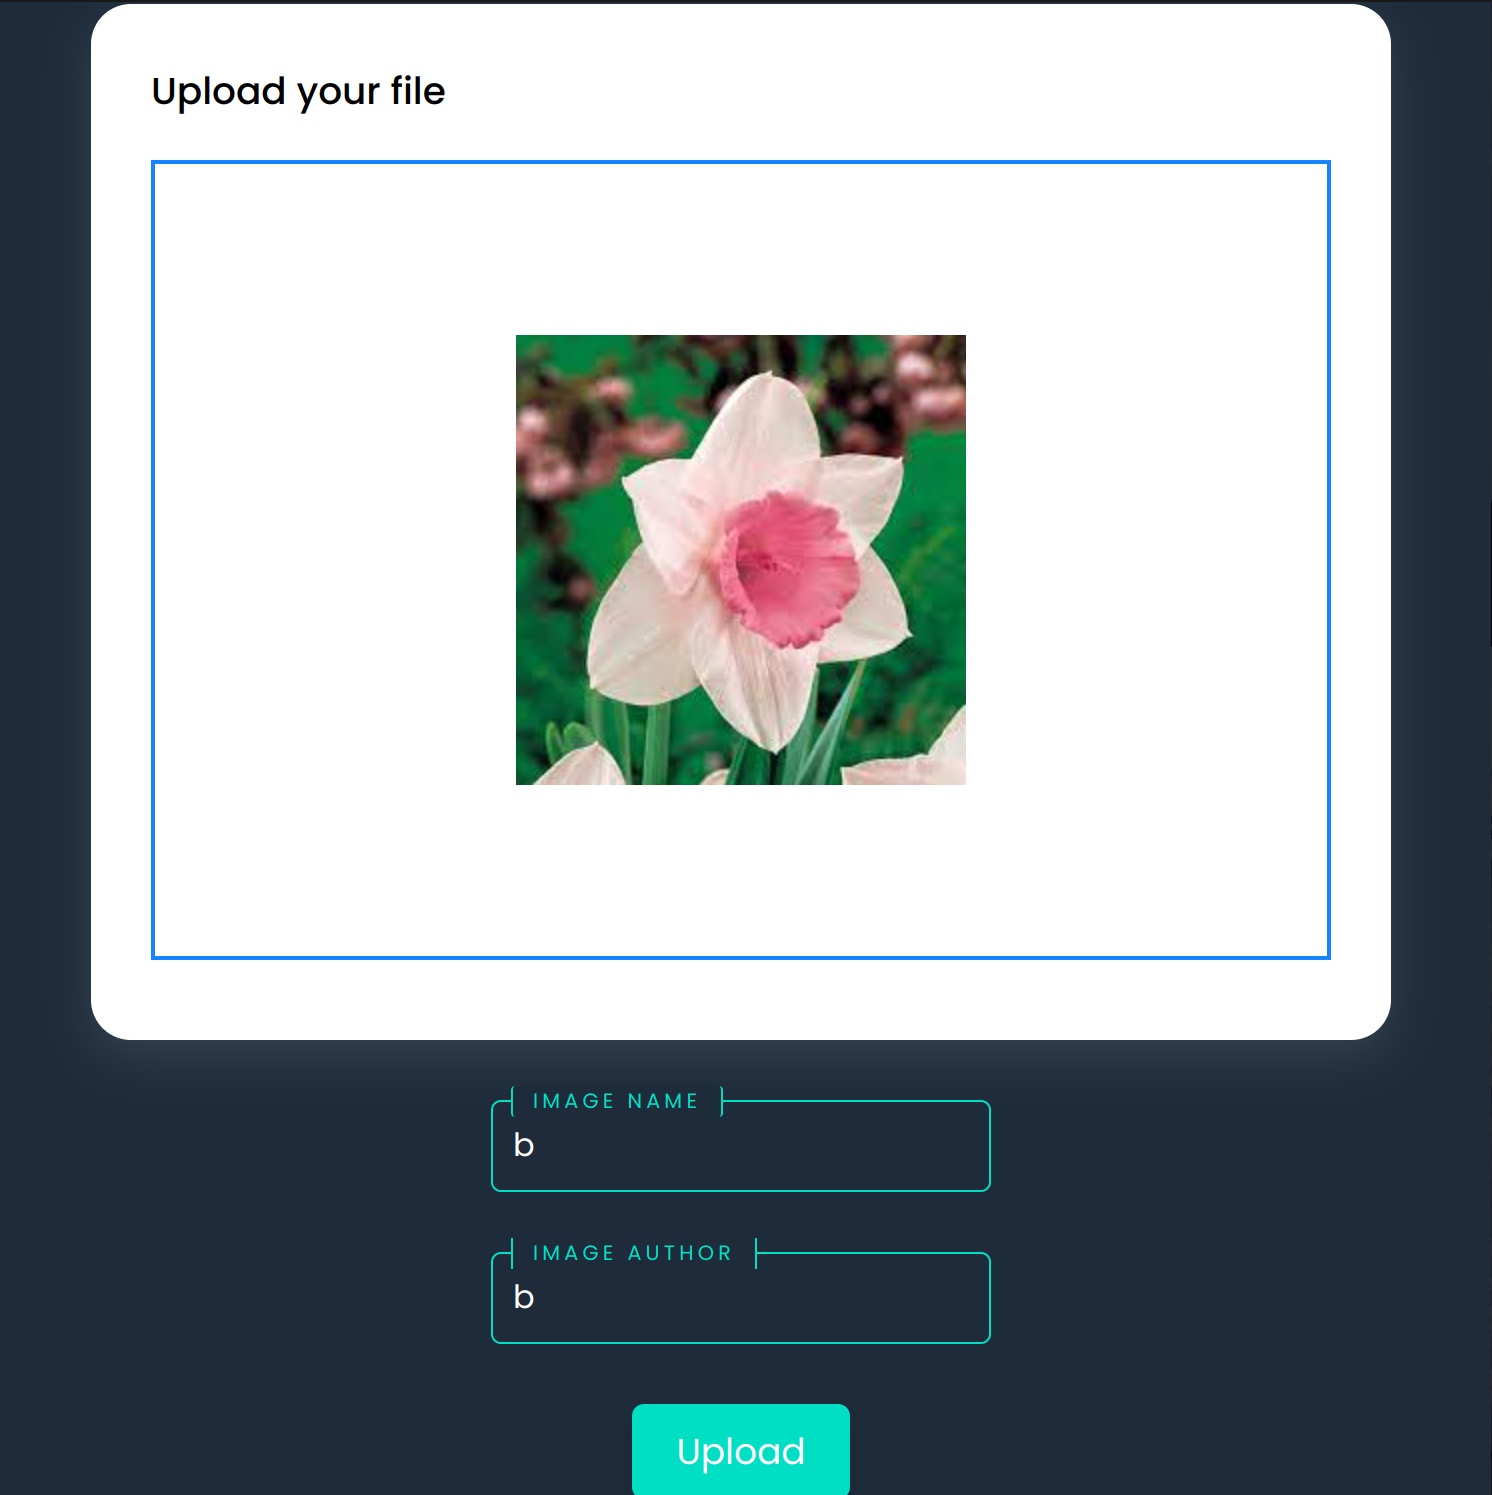
\includegraphics[scale=0.2]{../images/uploads}
    \caption{Pagina de uploads}
    \label{fig:uploads}
\end{figure}

\subsubsection{Profile}

\begin{figure}[H]
    \centering
    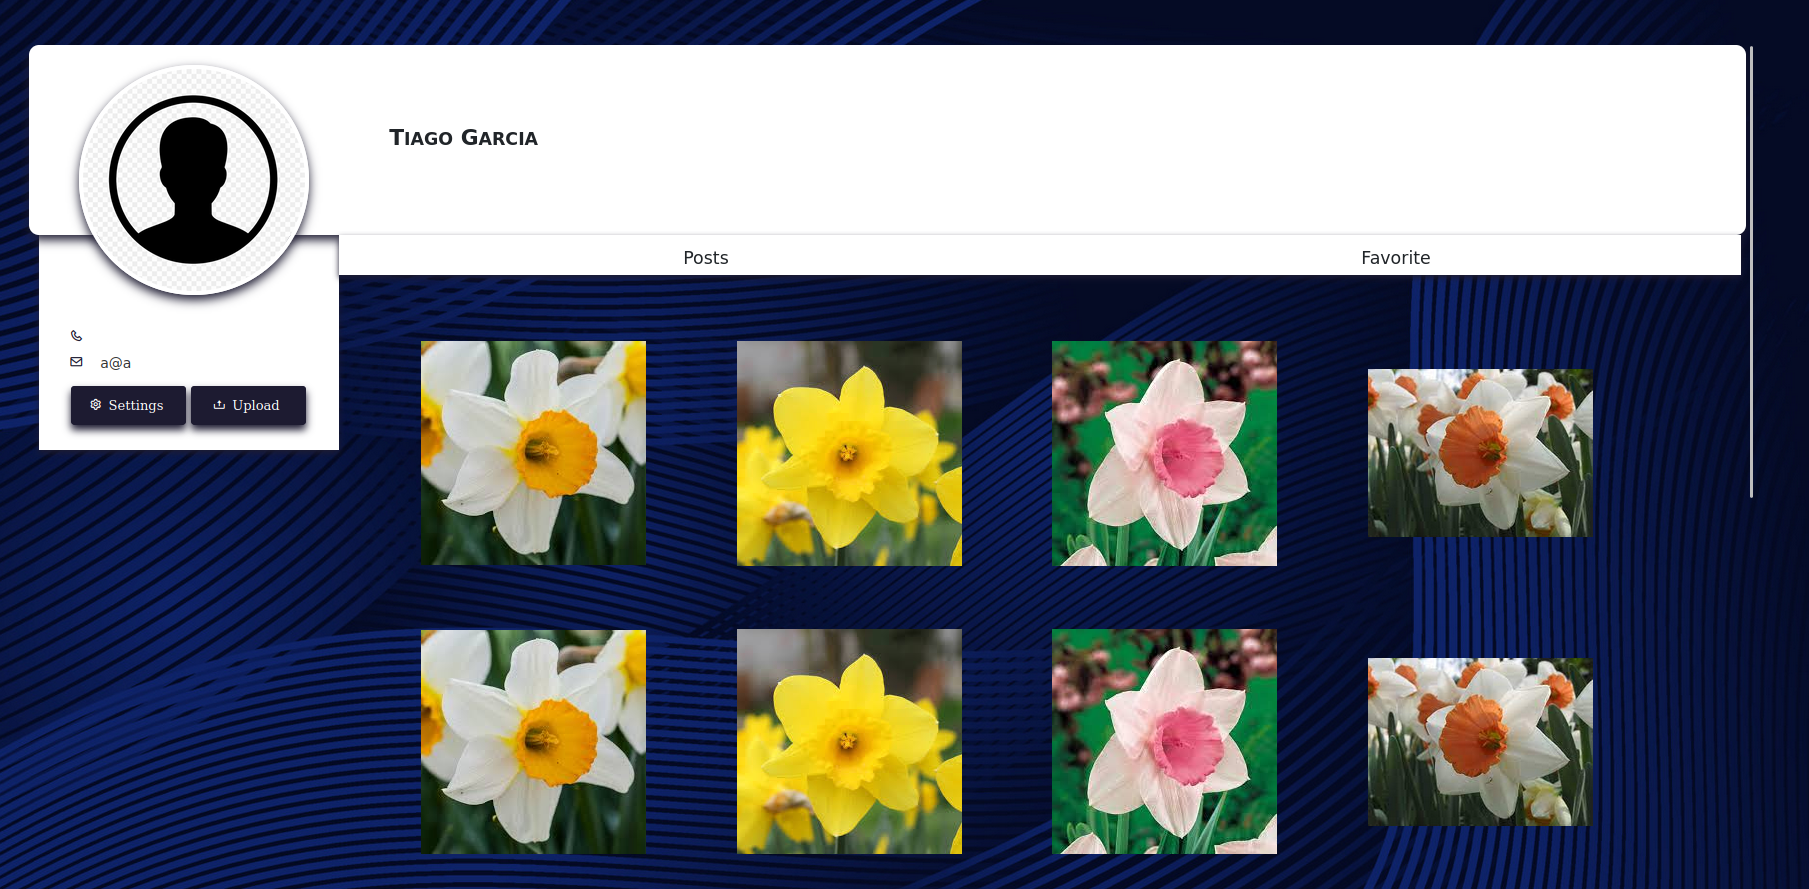
\includegraphics[scale=0.2]{../images/profile}
    \caption{Perfil}
    \label{fig:profile}
\end{figure}

\subsubsection{Image}

\begin{figure}[H]
    \centering
    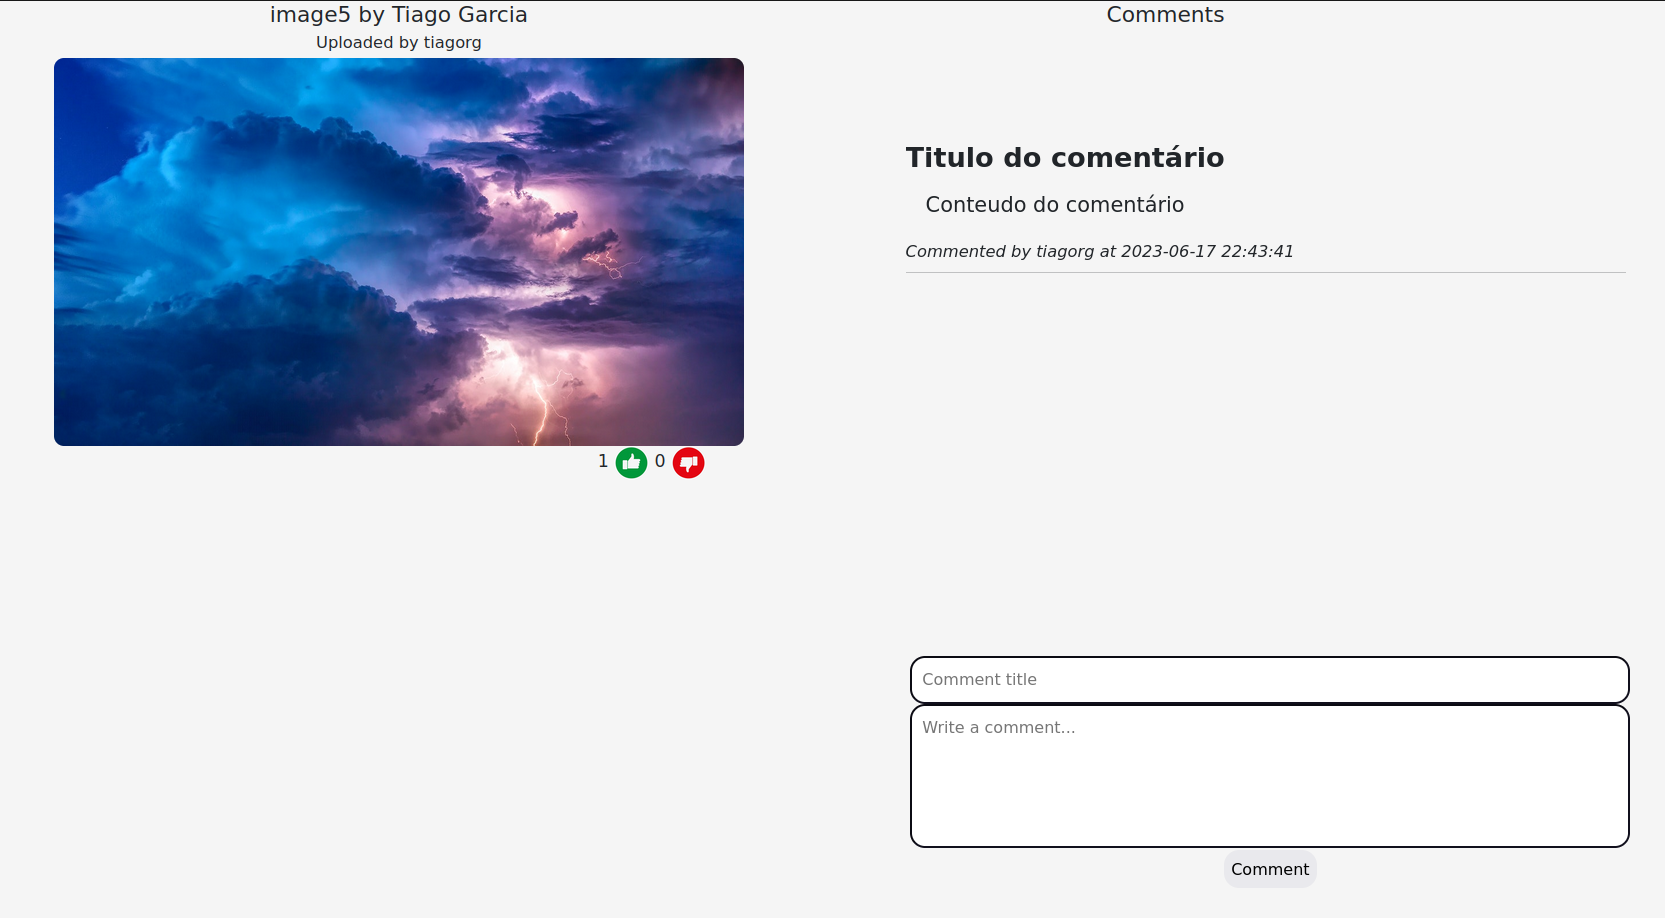
\includegraphics[scale=0.2]{../images/image}
    \caption{Pagina de uma imagem}
    \label{fig:image}
\end{figure}

\subsubsection{About}

\begin{figure}[H]
    \centering
    
\includegraphics[scale=0.2]{../images/About}
    \caption{Pagina de about}
    \label{fig:about}
\end{figure}

\section{Base de Dados}

\subsubsection{Users}

\begin{figure}[H]
    \centering
    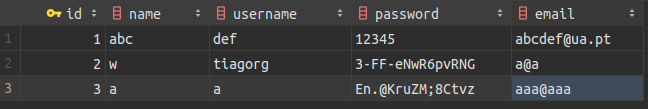
\includegraphics[scale=0.2]{../images/users}
    \caption{Tabela representante dos utilizadores}
    \label{fig:users}
\end{figure}

\subsubsection{Images.}

\begin{figure}[H]
    \centering
    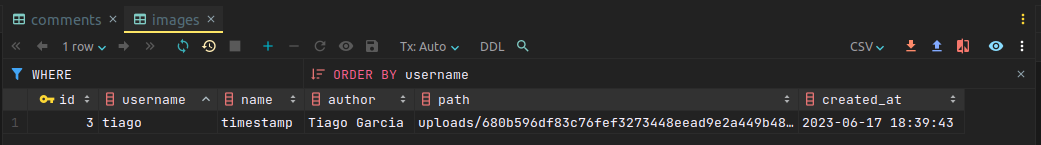
\includegraphics[scale=0.2]{../images/images}
    \caption{Tabela representante das imagens}
    \label{fig:images}
\end{figure}

\subsubsection{Votes}

\begin{figure}[H]
    \centering
    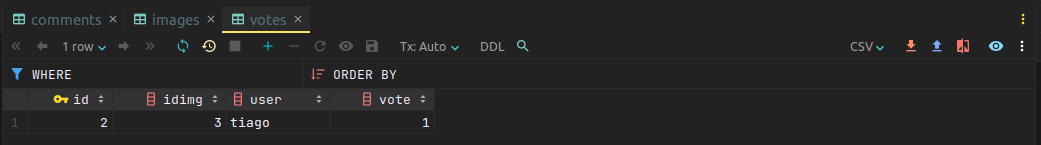
\includegraphics[scale=0.2]{../images/votes}
    \caption{Tabela representante dos likes/dislikes}
    \label{fig:votes}
\end{figure}

\subsubsection{Comments}

\begin{figure}[H]
    \centering
    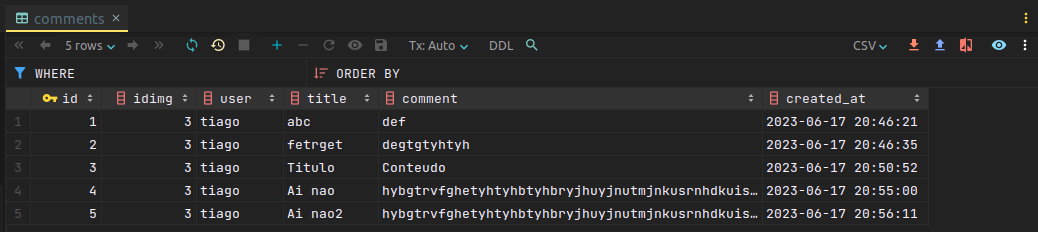
\includegraphics[scale=0.2]{../images/comments}
    \caption{Tabela representante dos comentários}
    \label{fig:comments}
\end{figure}

\chapter{Conclusões}
\label{chap.conclusao}
Com este projeto, foi possível desenvolver um site de partilha de imagens, onde é possível fazer \textit{upload} de imagens, comentar, e dar \textit{likes/dislikes} a imagens.\ O site foi desenvolvido com o objetivo de ser simples, e intuitivo, para que qualquer utilizador o consiga utilizar sem dificuldades.\ Os autores consideram que este projeto foi bastante abrangente, pois foi utilizado todo o conhecimento obtido nas cadeiras de \ac{labi} e \ac{iei}.\ O resultado obtido foi o esperado

\chapter*{Contribuições dos autores}
O trabalho de cada autor foi o seguinte:
\begin{itemize}
    \item \textbf{Bruno Pereira} - Desenvolvimento da base de dados e das páginas main, gallery (incluindo \ac{css} e \ac{js}), e eventuais ajustes em outras páginas.
    \item \textbf{Tiago Ferreira} - Desenvolvimento da página index e profile (incluindo \ac{css} e \ac{js}), e eventuais ajustes em outras páginas.\ Desenvolvimento do relatório.
    \item \textbf{Tiago Garcia} - Desenvolvimento da app e da página about, e grandes ajustes em outras páginas.
    \item \textbf{Rúben Gomes} - Desenvolvimento das páginas image, upload (incluindo \ac{css} e \ac{js}), e eventuais ajustes em outras páginas.\ Desenvolvimento do relatório.
\end{itemize}

\vspace{10pt}
\textbf{Percentagem de contribuição de cada autor.}\\

\autores : 25\%, 25\%, 25\%, 25\%\\

\textbf{Repositório GitHub:} labi2023g1

%%%%%%%%%%%%%%%%%%%%%%%%%%%%%%%%%
\chapter*{Acrónimos}
\begin{acronym}
    \acro{ua}[UA]{Universidade de Aveiro}
    \acro{leci}[LECI]{Licenciatura em Engenharia de Computadores e Informática}
    \acro{glisc}[GLISC]{Grey Literature International Steering Committee}
    \acro{json}[JSON]{JavaScript Object Notation}
    \acro{html}[HTML]{Hypertext Markup Language}
    \acro{css}[CSS]{Cascading Style Sheets}
    \acro{js}[JS]{JavaScript}
    \acro{sql}[SQL]{Structured Query Language}
    \acro{labi}[LABI]{Laboratórios de Informática}
    \acro{iei}[IEI]{Introdução à Engenharia Informática}
\end{acronym}


%%%%%%%%%%%%%%%%%%%%%%%%%%%%%%%%%
\printbibliography

\end{document}
